\clearpage
\fancyhead[R]{\sffamily\small\color{Muted}Vulkan / 光照实测}
\ctexset{section={afterindent=true},subsection={afterindent=true}}
\setlength{\parindent}{2\ccwd}
\section{Sponza 中庭的直接光与反射光}
看中庭地面上的一块石板。灯直接照到它，是直接光；灯先照亮柱子，柱子再把光反射到石板上，才算一次间接光。程序把这两部分分开保存。直接光有亮度较高的局部光斑，反射光弱得多，能照到灯光够不到的地方。

\begin{figure}[H]\centering
\panelimage{.48\linewidth}{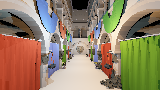
\includegraphics[width=\linewidth]{gi/direct-reference.png}}{16 盏灯逐一求和}
\hfill
\panelimage{.48\linewidth}{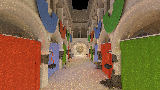
\includegraphics[width=\linewidth]{gi/indirect-reference.png}}{只保留一次反射}
\caption{同一机位、同一套线性材质。为看清较弱的反射，右图显示曝光为 20，左图为 4。下文的误差均从调曝光前的浮点值计算。}
\end{figure}

场景来自 Khronos 示例资产库。测试把 Sponza 的最长边缩放到 20 个场景单位，在通道两侧放置 16 盏暖色和冷色点光。相机位于 $(-5.5,-2.2,0)$，朝向 $(6,-1.8,0)$，垂直视角 $65^\circ$。GPU 用包围盒树查找射线先碰到哪块三角形。为了只比较光照估计，基准里的每个材质用底色贴图的平均线性反射率，忽略透明裁剪，两个方向都能击中三角形。

直接光的对照逐一检查每盏灯能否照到石板，然后把可见灯的贡献加起来。间接光需要知道周围每个方向反射回来多少光。对照为每个可见像素发出两组各 512 条半球射线。每条射线击中另一块表面后，采样一盏灯并检查中间有无遮挡；把两组独立结果平均，得到每像素 1,024 个样本的参考图。两组结果的差异给出约 $1.08\times10^{-5}$ 的参考均方误差估计，参考图本身仍有噪声。

误差在 $160\times90$ 图中的 14,256 个可见像素上计算。对每个像素和三个颜色通道，把测量值减去对应参考值，平方后取平均。这个数越小，说明颜色越接近同一张参考图。实验使用四个随机种子，各种方法共用同一组种子。灯、镜头和几何保持静止。

\readings{\refitem{https://github.com/KhronosGroup/glTF-Sample-Assets/tree/e124e8d8d7330a5372bc2b4d00d39a4a9d7997ea/Models/Sponza}{Khronos · Sponza 模型来源与作者}。\texttt{tests/fetch\_sponza.py} 下载同一版本。}

\clearpage
\section{样本怎样影响亮度与误差}
直接光最简单的近似是每次选一盏灯。若恰好选了柱子后面的灯，这个像素本帧就得零。ReSTIR DI 会把自己的新候选与上一帧、相邻像素的候选一起比较。保留下来的记录叫作样本库（reservoir），里面只存一个选中的候选、累计权重和候选数。来自邻居的灯仍需从当前表面重新检查阴影。下面的 DI 和 GI 每帧每个可见像素各产生一个新候选，另检查最多四个邻居，表中读取运行八帧后的输出。

间接光可以从两条路近似。DDGI 在房间里布置 $12\times6\times7$ 个探针，每个探针向六个朝向分别取 16 条射线，记录反射光和到障碍物的距离。石板从附近八个探针插值，再乘上自身反射率。ReSTIR GI 保存的是光从其他表面反射过来的那段路径。邻像素用到这条路径时，需要重新检查石板能否看见第二块表面，再按新连线的距离与两端角度计算贡献。因此，同一盏灯被柱子挡住与同一段反射路径被柱子挡住，涉及两种不同的可见性检查。

{\noindent\smalltable\begin{tabularx}{\linewidth}{@{}Xrrr@{}}\toprule
估计方法 & 均方误差 & 平均线性 RGB & 复用占比\\\midrule
直接光，每像素 1 个样本 & 0.16609 & 0.10873 & ---\\
直接光，每像素 8 个样本 & 0.02152 & 0.11019 & ---\\
ReSTIR DI，第 8 帧 & 0.01132 & 0.11226 & 91.0\%\\\midrule
反射光，每像素 1 个样本 & 0.02238 & 0.01148 & ---\\
反射光，每像素 8 个样本 & 0.001810 & 0.01115 & ---\\
DDGI，第 8 帧 & 0.0000410 & 0.00904 & ---\\
ReSTIR GI，第 8 帧 & 0.0003678 & 0.01017 & 91.6\%\\\bottomrule
\end{tabularx}\par}

复用占比统计全部可见像素中，最终选中已有候选且确实有光的比例。直接光参考平均为 0.11140，反射光为 0.01110。探针得到的反射光最平滑，平均亮度也比参考低约 18.5\%；ReSTIR GI 低约 8.4\%。表中的每种方法承担的工作不同。探针试验每帧会更新全部探针，样本复用也要付出重新检查遮挡的成本。仅凭误差无法比较每毫秒画出的效果。

\readings{论文与实现范围可对照 \refitem{https://research.nvidia.com/publication/2019-05_dynamic-diffuse-global-illumination-ray-traced-irradiance-fields}{Majercik 等 · DDGI}、
\refitem{https://research.nvidia.com/labs/rtr/publication/bitterli2020spatiotemporal/}{Bitterli 等 · ReSTIR DI} 与
\refitem{https://research.nvidia.com/publication/2021-06_restir-gi-path-resampling-real-time-path-tracing}{Ouyang 等 · ReSTIR GI}。本次实现只测单次漫反射，探针使用六个朝向，样本复用使用有限历史和兼容表面筛选。}

\clearpage
\section{在 RenderDoc 里找回这三种光照}
打开 \path{SponzaGI_capture.rdc}，先选事件 8，再选事件 20。前者把新采到的反射光写入探针，后者按每个可见表面的位置读取相邻探针。接着看事件 44 和 68。它们写同一份像素缓冲区，里面在这两个时刻分别存着直接光和一次反射光。回放脚本分别停在这三个输出时刻，读出每像素四个浮点数，用前三个数生成了下图。

\begin{figure}[H]\centering
\panelimage{.318\linewidth}{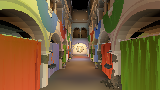
\includegraphics[width=\linewidth]{gi/capture-ddgi.png}}{20 · 探针反射光}
\hfill\panelimage{.318\linewidth}{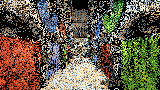
\includegraphics[width=\linewidth]{gi/capture-di.png}}{44 · 直接光}
\hfill\panelimage{.318\linewidth}{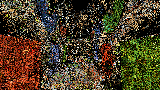
\includegraphics[width=\linewidth]{gi/capture-gi.png}}{68 · 路径反射光}
\caption{RenderDoc 1.47 的首帧回放。第三幅还有明显颗粒。本次捕获从空历史开始；上一页比较的两种 ReSTIR 结果已经运行八帧。}
\end{figure}

{\noindent\smalltable\begin{tabularx}{\linewidth}{@{}Xrrrr@{}}\toprule
GPU 执行内容 & 事件 & 工作组数 & 中位数（ms） & 范围（ms）\\\midrule
\giTimingRows\bottomrule\end{tabularx}\par}

在 RTX 5070 Ti Laptop GPU 上先回放一次预热，再读取九轮 RenderDoc 的 GPU 事件计时。每组有 64 个线程，225 组覆盖一整张图。计时只覆盖表中相应的一条计算命令。工程启用 Debug/x64，独立基准的 CPU 计时还包含命令记录、提交和等待，原始数据单列于 \path{trials.csv}。这两种时间都不能直接换算成编辑器帧率。

探针更新明显比在表面查询探针耗时。下一轮可以每次只更新部分探针，把节省的毫秒与移动光源后的追光延迟放在一起比较。另一项可复现实验是固定总 GPU 毫秒，改变反射路径的邻居数，观察柱脚附近的噪声与平均亮度是否改善。这样才能检验增加复用是否值得。

\readings{原始帧、独立结果和逐事件回放记录保存在 \path{output/profiling/gi/}。运行 \path{tests/run_gi_benchmark.cmd} 与 \path{tests/analyze_gi.py} 可重算误差。探针与路径的实现见 \path{GI/Shaders/GI.comp}。}

\clearpage
\section{镜头停下后，哪些像素还在变}
编辑器里曾出现这样的现象：相机已经停下，远处的线条还在晃。为分开检查成因，这组实验改用编辑器场景里的三盏点光和模型纹理，固定 Sponza 的变换与镜头，按旧版预览的 $320\times180$ 连续生成 24 帧。这里可以分别关闭光照采样和相机的亚像素偏移，再看某个像素下一帧究竟变了多少。

\begin{figure}[H]\centering
\panelimage{.318\linewidth}{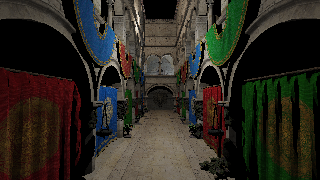
\includegraphics[width=\linewidth]{gi/temporal-static-direct.png}}{固定相机 · 三盏场景灯}
\hfill\panelimage{.318\linewidth}{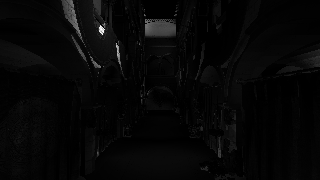
\includegraphics[width=\linewidth]{gi/temporal-ddgi-2-change.png}}{只引入低样本探针}
\hfill\panelimage{.318\linewidth}{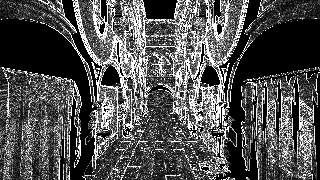
\includegraphics[width=\linewidth]{gi/temporal-direct-jitter-change.png}}{只偏移直接光采样点}
\caption{后两图比较第 23 与第 24 帧，取 RGB 三个通道中最大的显示差，再放大八倍。白色靠近变化较大的区域。右图的屋顶、布帘和纹理边缘都跟着采样位置改变。}
\end{figure}

先画逐盏计算的直接光。固定投影时，这 24 帧逐值相同；在同一个相机上只改变每帧采样点，全图有 60.89\% 的像素出现超过 3 个显示色阶的相邻帧差。这里尚未混合 TAA，测量的是它收到的输入。旧设置还把宽 320 像素的结果放大到整个面板，像素和细节一起被放大。

再固定投影，只让采样算法继续工作。将直接光和 DDGI 的一次反射相加，使用面板相同的显示曲线。每个探针方向发两条射线时，有 3.89\% 的像素变化超过同一门槛；增加到 16 条，降到 1.03\%。换成 ReSTIR GI 后为 9.31\%。单独显示 ReSTIR DI 时为 28.49\%。这些比例取第 9 至 24 帧的 15 对相邻画面，任一颜色通道从 0 至 255 的值相差超过 3 即计入一次。

这 24 帧中，每种算法记录的帧数都从 1 加到了 24，中途没有重新计数。镜头不动时，墙面仍可能因每帧只取少量光线而忽明忽暗。要检查这种抖动，可以先用面板的原始分辨率固定相机，再分别比较 TAA 混合前后的两帧。独立测试也把尺寸从 $320\times180$ 改成 $319\times179$ 再还原，逐像素核对固定相机输出和三盏灯，结果一致。

\readings{运行 \path{tests/run_gi_benchmark.cmd --temporal} 与 \path{tests/analyze_gi_temporal.py} 可重算。测量与逐帧变化图见 \path{output/profiling/gi/temporal.json} 及同目录 PNG。}
